\documentclass[11pt,a4paper,]{article}
\usepackage{lmodern}

\usepackage{amssymb,amsmath}
\usepackage{ifxetex,ifluatex}
\usepackage{fixltx2e} % provides \textsubscript
\ifnum 0\ifxetex 1\fi\ifluatex 1\fi=0 % if pdftex
  \usepackage[T1]{fontenc}
  \usepackage[utf8]{inputenc}
\else % if luatex or xelatex
  \usepackage{unicode-math}
  \defaultfontfeatures{Ligatures=TeX,Scale=MatchLowercase}
\fi
% use upquote if available, for straight quotes in verbatim environments
\IfFileExists{upquote.sty}{\usepackage{upquote}}{}
% use microtype if available
\IfFileExists{microtype.sty}{%
\usepackage[]{microtype}
\UseMicrotypeSet[protrusion]{basicmath} % disable protrusion for tt fonts
}{}
\PassOptionsToPackage{hyphens}{url} % url is loaded by hyperref
\usepackage[unicode=true]{hyperref}
\hypersetup{
            pdftitle={Research on COVID-19 and vaccination},
            pdfborder={0 0 0},
            breaklinks=true}
\urlstyle{same}  % don't use monospace font for urls
\usepackage{geometry}
\geometry{a4paper, centering, text={16cm,24cm}}
\usepackage[style=authoryear-comp,]{biblatex}
\addbibresource{references.bib}
\usepackage{longtable,booktabs}
% Fix footnotes in tables (requires footnote package)
\IfFileExists{footnote.sty}{\usepackage{footnote}\makesavenoteenv{long table}}{}
\IfFileExists{parskip.sty}{%
\usepackage{parskip}
}{% else
\setlength{\parindent}{0pt}
\setlength{\parskip}{6pt plus 2pt minus 1pt}
}
\setlength{\emergencystretch}{3em}  % prevent overfull lines
\providecommand{\tightlist}{%
  \setlength{\itemsep}{0pt}\setlength{\parskip}{0pt}}
\setcounter{secnumdepth}{5}

% set default figure placement to htbp
\makeatletter
\def\fps@figure{htbp}
\makeatother


\title{Research on COVID-19 and vaccination}

%% MONASH STUFF

%% CAPTIONS
\RequirePackage{caption}
\DeclareCaptionStyle{italic}[justification=centering]
 {labelfont={bf},textfont={it},labelsep=colon}
\captionsetup[figure]{style=italic,format=hang,singlelinecheck=true}
\captionsetup[table]{style=italic,format=hang,singlelinecheck=true}


%% FONT
\RequirePackage{bera}
\RequirePackage[charter,expert,sfscaled]{mathdesign}
\RequirePackage{fontawesome}

%% HEADERS AND FOOTERS
\RequirePackage{fancyhdr}
\pagestyle{fancy}
\rfoot{\Large\sffamily\raisebox{-0.1cm}{\textbf{\thepage}}}
\makeatletter
\lhead{\textsf{\expandafter{\@title}}}
\makeatother
\rhead{}
\cfoot{}
\setlength{\headheight}{15pt}
\renewcommand{\headrulewidth}{0.4pt}
\renewcommand{\footrulewidth}{0.4pt}
\fancypagestyle{plain}{%
\fancyhf{} % clear all header and footer fields
\fancyfoot[C]{\sffamily\thepage} % except the center
\renewcommand{\headrulewidth}{0pt}
\renewcommand{\footrulewidth}{0pt}}

%% MATHS
\RequirePackage{bm,amsmath}
\allowdisplaybreaks

%% GRAPHICS
\RequirePackage{graphicx}
\setcounter{topnumber}{2}
\setcounter{bottomnumber}{2}
\setcounter{totalnumber}{4}
\renewcommand{\topfraction}{0.85}
\renewcommand{\bottomfraction}{0.85}
\renewcommand{\textfraction}{0.15}
\renewcommand{\floatpagefraction}{0.8}


%\RequirePackage[section]{placeins}

%% SECTION TITLES


%% SECTION TITLES (NEW: Changing sections and subsections color)
\RequirePackage[compact,sf,bf]{titlesec}
\titleformat*{\section}{\Large\sf\bfseries\color[rgb]{0.8, 0.7, 0.1 }}
\titleformat*{\subsection}{\large\sf\bfseries\color[rgb]{0.8, 0.7, 0.1 }}
\titleformat*{\subsubsection}{\sf\bfseries\color[rgb]{0.8, 0.7, 0.1 }}
\titlespacing{\section}{0pt}{2ex}{.5ex}
\titlespacing{\subsection}{0pt}{1.5ex}{0ex}
\titlespacing{\subsubsection}{0pt}{.5ex}{0ex}


%% TITLE PAGE
\def\Date{\number\day}
\def\Month{\ifcase\month\or
 January\or February\or March\or April\or May\or June\or
 July\or August\or September\or October\or November\or December\fi}
\def\Year{\number\year}

%% LINE AND PAGE BREAKING
\sloppy
\clubpenalty = 10000
\widowpenalty = 10000
\brokenpenalty = 10000
\RequirePackage{microtype}

%% PARAGRAPH BREAKS
\setlength{\parskip}{1.4ex}
\setlength{\parindent}{0em}

%% HYPERLINKS
\RequirePackage{xcolor} % Needed for links
\definecolor{darkblue}{rgb}{0,0,.6}
\RequirePackage{url}

\makeatletter
\@ifpackageloaded{hyperref}{}{\RequirePackage{hyperref}}
\makeatother
\hypersetup{
     citecolor=0 0 0,
     breaklinks=true,
     bookmarksopen=true,
     bookmarksnumbered=true,
     linkcolor=darkblue,
     urlcolor=blue,
     citecolor=darkblue,
     colorlinks=true}

\usepackage[showonlyrefs]{mathtools}
\usepackage[no-weekday]{eukdate}

%% BIBLIOGRAPHY

\makeatletter
\@ifpackageloaded{biblatex}{}{\usepackage[style=authoryear-comp, backend=biber, natbib=true]{biblatex}}
\makeatother
\ExecuteBibliographyOptions{bibencoding=utf8,minnames=1,maxnames=3, maxbibnames=99,dashed=false,terseinits=true,giveninits=true,uniquename=false,uniquelist=false,doi=false, isbn=false,url=true,sortcites=false}

\DeclareFieldFormat{url}{\texttt{\url{#1}}}
\DeclareFieldFormat[article]{pages}{#1}
\DeclareFieldFormat[inproceedings]{pages}{\lowercase{pp.}#1}
\DeclareFieldFormat[incollection]{pages}{\lowercase{pp.}#1}
\DeclareFieldFormat[article]{volume}{\mkbibbold{#1}}
\DeclareFieldFormat[article]{number}{\mkbibparens{#1}}
\DeclareFieldFormat[article]{title}{\MakeCapital{#1}}
\DeclareFieldFormat[article]{url}{}
%\DeclareFieldFormat[book]{url}{}
%\DeclareFieldFormat[inbook]{url}{}
%\DeclareFieldFormat[incollection]{url}{}
%\DeclareFieldFormat[inproceedings]{url}{}
\DeclareFieldFormat[inproceedings]{title}{#1}
\DeclareFieldFormat{shorthandwidth}{#1}
%\DeclareFieldFormat{extrayear}{}
% No dot before number of articles
\usepackage{xpatch}
\xpatchbibmacro{volume+number+eid}{\setunit*{\adddot}}{}{}{}
% Remove In: for an article.
\renewbibmacro{in:}{%
  \ifentrytype{article}{}{%
  \printtext{\bibstring{in}\intitlepunct}}}

\AtEveryBibitem{\clearfield{month}}
\AtEveryCitekey{\clearfield{month}}

\makeatletter
\DeclareDelimFormat[cbx@textcite]{nameyeardelim}{\addspace}
\makeatother

\author{\sf\Large\textbf{ Krisanat Anukarnsakulchularp}\\ {\sf\large Master of Business Analytics\\[0.5cm]} \sf\Large\textbf{ Kumar Vatsal}\\ {\sf\large Master of Business Analytics\\[0.5cm]} \sf\Large\textbf{ Xiyun Zhou}\\ {\sf\large Master of Actuarial Studies\\[0.5cm]} \sf\Large\textbf{ Xinyu Hu}\\ {\sf\large Master of Applied Economics and Econometrics\\[0.5cm]}}

\date{\sf\Date~\Month~\Year}
\makeatletter
\lfoot{\sf Anukarnsakulchularp, Vatsal, Zhou, Hu: \@date}
\makeatother


%%%% PAGE STYLE FOR FRONT PAGE OF REPORTS

\makeatletter
\def\organization#1{\gdef\@organization{#1}}
\def\telephone#1{\gdef\@telephone{#1}}
\def\email#1{\gdef\@email{#1}}
\makeatother
  \organization{Monash University}

  \def\name{ETC5513\newline Quad Squad}

  \telephone{(03) 9905 2478}

  \email{questions@company.com}                 %NEW: New email addresss

\def\webaddress{\url{http://company.com/stats/consulting/}} %NEW: URl
\def\abn{12 377 614 630}                                    % NEW: ABN
\def\logo{
\includegraphics[width=6cm]{Figures/logo}}  %NEW: Changing logo
\def\extraspace{\vspace*{1.6cm}}
\makeatletter
\def\contactdetails{\faicon{phone} & \@telephone \\
                    \faicon{envelope} & \@email}
\makeatother

%%%% FRONT PAGE OF REPORTS

\def\reporttype{Report for}

\long\def\front#1#2#3{
\newpage
\begin{singlespacing}
\thispagestyle{empty}
\vspace*{-1.4cm}
\hspace*{-1.4cm}
\hbox to 16cm{
  \hbox to 6.5cm{\vbox to 14cm{\vbox to 25cm{
    \logo
    \vfill
    \parbox{6.3cm}{\raggedright
      \sf\color[rgb]{0.8, 0.7, 0.1 }    % NEW color 
      {\large\textbf{\name}}\par
      \vspace{.7cm}
      \tabcolsep=0.12cm\sf\small
      \begin{tabular}{@{}ll@{}}\contactdetails
      \end{tabular}
      \vspace*{0.3cm}\par
      ABN: \abn\par
    }
  }\vss}\hss}
  \hspace*{0.2cm}
  \hbox to 1cm{\vbox to 14cm{\rule{4pt}{26.8cm}\vss}\hss\hfill}  %NEW: Thicker line
  \hbox to 10cm{\vbox to 14cm{\vbox to 25cm{   
      \vspace*{3cm}\sf\raggedright
      \parbox{11cm}{\sf\raggedright\baselineskip=1.2cm
         \fontsize{24.88}{30}\color[rgb]{0, 0.29, 0.55}\sf\textbf{#1}}   % NEW: title color blue
      \par
      \vfill
      \large
      \vbox{\parskip=0.8cm #2}\par
      \vspace*{2cm}\par
      \reporttype\\[0.3cm]
      \hbox{#3}%\\[2cm]\
      \vspace*{1cm}
      {\large\sf\textbf{\Date~\Month~\Year}}
   }\vss}
  }}
\end{singlespacing}
\newpage
}

\makeatletter
\def\titlepage{\front{\expandafter{\@title}}{\@author}{\@organization}}
\makeatother

\usepackage{setspace}
\setstretch{1.5}

%% Any special functions or other packages can be loaded here.
\usepackage{booktabs}
\usepackage{longtable}
\usepackage{array}
\usepackage{multirow}
\usepackage{wrapfig}
\usepackage{float}
\usepackage{colortbl}
\usepackage{pdflscape}
\usepackage{tabu}
\usepackage{threeparttable}
\usepackage{threeparttablex}
\usepackage[normalem]{ulem}
\usepackage{makecell}
\usepackage{xcolor}


\begin{document}
\titlepage

\clearpage

\hypertarget{introduction}{%
\section{\texorpdfstring{\textbf{Introduction}}{Introduction}}\label{introduction}}

Since the first outbreak of Covid-19 in late 2019, there have been more than 500 million confirmed cases. To curb the spread, governments around the world had taken several measures like imposing restrictions on travelling, lockdown, and introducing social-distance.

To bring this pandemic to an end, a large share of the world needs to be immune to the virus. The safest way to achieve this is with a vaccine. Vaccines are a technology that humanity has often relied on in the past to bring down the death toll of infectious diseases.

Fortunately in 2021, COVID-19 vaccines were introduced, it would require an incredibly-high vaccination rate to reduce the spread of the virus. Although the vaccines are not able to prevent infection, yet they are efficient at keeping the mortality rate low. ``You may wonder if the vaccine is so effective, why are we still having a growth in the infection rate.''

We collected data from a public data base in github \href{https://github.com/owid/covid-19-data/tree/master/public/data}{COVID-19 data}. In this report, we focus on overall COVID-19 analysis and explore the relationship between the pandemic and the vaccination by the world range.

The packages we will be using in this analysis are bookdown (\textcite{bookdown}), readr (\textcite{readr}), kableExtra (\textcite{kableExtra}), ggplot2 (\textcite{ggplot2}), tidyverse (\textcite{tidyverse}), and lubridate (\textcite{lubridate})

\clearpage

\hypertarget{research-questions}{%
\section{\texorpdfstring{\textbf{Research questions} :}{Research questions :}}\label{research-questions}}

With the introduction of the COVID-19 vaccines, we want to see whether the use of vaccines or the use of the restriction will be better at fighting against COVID-19?

The report will be divided into different sections to explore the research question.

\begin{enumerate}
\def\labelenumi{(\arabic{enumi})}
\item
  \textbf{The overall analysis of COVID-19.}
\item
  \textbf{The Effects of government policies on the spread of COVID- 19 worldwide.}
\item
  \textbf{How do positive cases change relate to vaccination?}
\item
  \textbf{How do death rates from COVID-19 differ between people who are vaccinated and those who are not?}
\end{enumerate}

\clearpage

\hypertarget{exploratory-data-analysis}{%
\section{\texorpdfstring{\textbf{Exploratory data analysis}}{Exploratory data analysis}}\label{exploratory-data-analysis}}

\hypertarget{the-overall-analysis-of-covid-19}{%
\subsection{\texorpdfstring{\textbf{The overall analysis of covid-19}}{The overall analysis of covid-19}}\label{the-overall-analysis-of-covid-19}}

\begin{figure}

{\centering 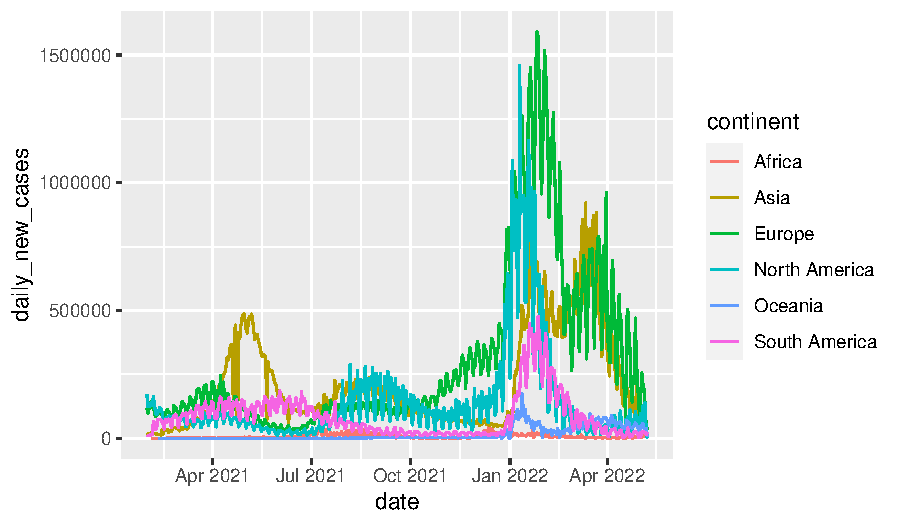
\includegraphics{report_files/figure-latex/Figure1-1} 

}

\caption{COVID-19 Daily new cases}\label{fig:Figure1}
\end{figure}

The line chart \ref{fig:Figure1} indicate from January 2021 to May 2022, the daily new cases show an upward trend. There are 3 times breakout in most regions, which occurs in the May 2021, August 2021, and February 2022. Especially in the past few months, the average daily cases reach to the highest point. Some countries in Europe and North America region have more than 1 million new cases every day. And European countries always have the highest daily cases in this period.

\begin{table}[!h]

\caption{\label{tab:Table1}Countries with Highest Average Daily Cases}
\centering
\begin{tabular}[t]{l|r}
\hline
location & average daily cases\\
\hline
\cellcolor{gray!6}{United States} & \cellcolor{gray!6}{120485}\\
\hline
India & 70729\\
\hline
\cellcolor{gray!6}{France} & \cellcolor{gray!6}{56649}\\
\hline
Germany & 50097\\
\hline
\cellcolor{gray!6}{Brazil} & \cellcolor{gray!6}{46861}\\
\hline
\end{tabular}
\end{table}

Table \ref{tab:Table1} list the top 5 countries with the highest average daily cases. The average daily cases are more than 1 million in United State.
In the following, the countries in the table will be utilised to examine the relationship between vaccination and daily new cases.

\begin{figure}

{\centering 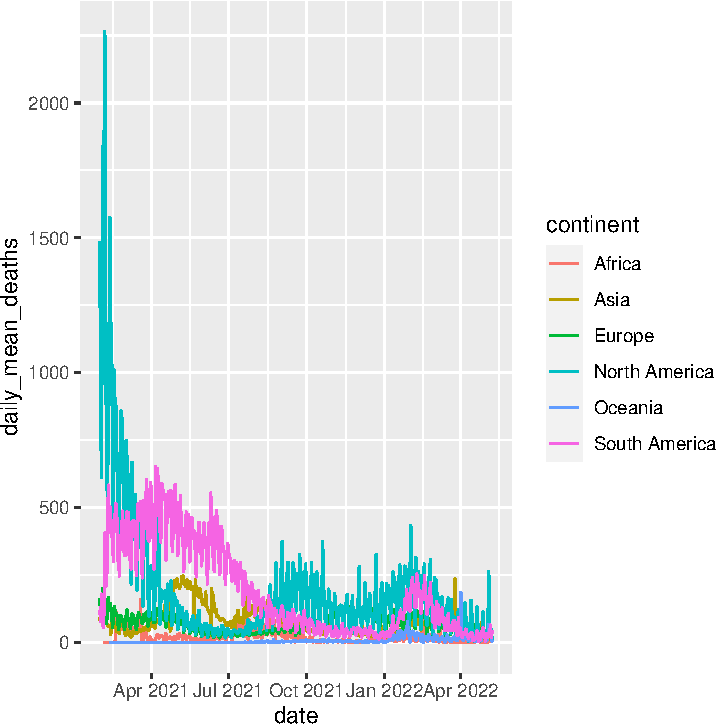
\includegraphics{report_files/figure-latex/Figure2-1} 

}

\caption{Average daily deaths attributed to COVID-19}\label{fig:Figure2}
\end{figure}

The overall of graph \ref{fig:Figure2} show a decline trend of average daily deaths attributed to COVID-19. The North America area has the greatest daily deaths in early 2021, and then the number of deaths drops dramatically beginning in May 2021. After October 2021, the average daily death toll in North America never exceed 500.

\begin{table}[!h]

\caption{\label{tab:Table2}COVID-19 Highest Average Daily Deaths Countries}
\centering
\begin{tabular}[t]{l|r}
\hline
location & average daily deaths\\
\hline
\cellcolor{gray!6}{United States} & \cellcolor{gray!6}{1201}\\
\hline
Brazil & 978\\
\hline
\cellcolor{gray!6}{India} & \cellcolor{gray!6}{798}\\
\hline
Russia & 662\\
\hline
\cellcolor{gray!6}{Mexico} & \cellcolor{gray!6}{396}\\
\hline
\end{tabular}
\end{table}

Table \ref{tab:Table2} list the top 5 countries with the highest average daily deaths caused by COVID-19.
In the following, the countries in the table will be using to analyse the relationship between vaccination and daily deaths.

\clearpage

\begin{figure}

{\centering 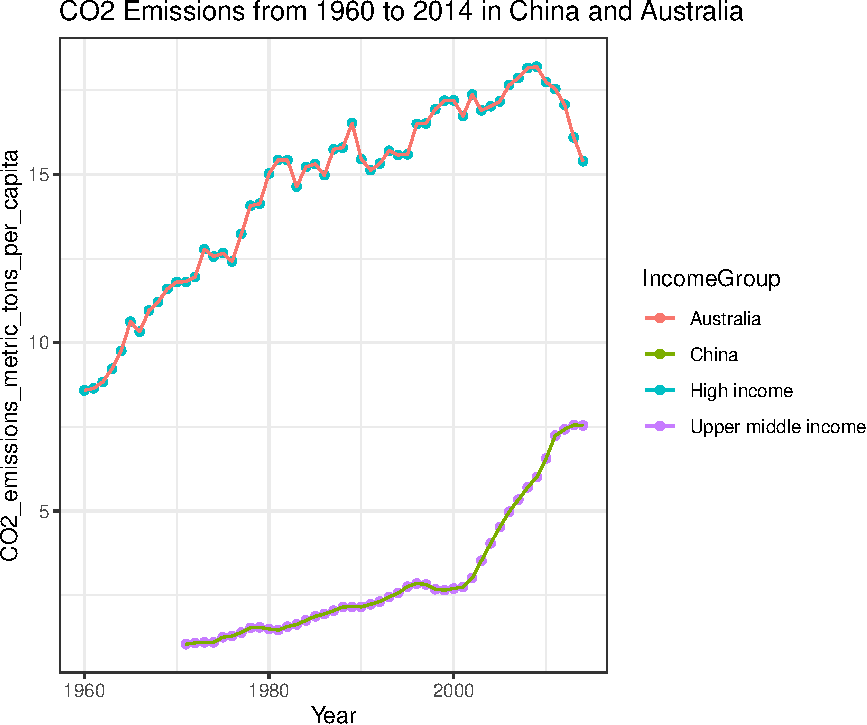
\includegraphics{report_files/figure-latex/Figure3-1} 

}

\caption{People fully vaccinated in percentage by region}\label{fig:Figure3}
\end{figure}

The barplot \ref{fig:Figure3} shows the fully vaccination rate by regions. Except Africa region, the fully vaccinated rate over 50\% in other continent. According to the research \textcite{African-COVID-19-vaccination}, at the end of December 2021, only 7 African countries with relatively smaller populations (Seychelles, Mauritius, Morocco, Tunisia, Comoros, Botswana, and Cape Verde) met the 40\% target. The African continent's fundamentally deficient health systems are undoubtedly leading to insufficient COVID-19 vaccination capability.

\clearpage

\hypertarget{effects-of-government-policies-on-the-spread-of-covid-19-worldwide}{%
\subsection{\texorpdfstring{\textbf{Effects of government policies on the spread of COVID-19 worldwide}}{Effects of government policies on the spread of COVID-19 worldwide}}\label{effects-of-government-policies-on-the-spread-of-covid-19-worldwide}}

\subsection*{Stringency Index}

Before the availability of the vaccination, the most commons measures against the COVID-19 is the use of restrictions implemented by the government. The Oxford Covid-19 Government Response Tracker (\textcite{OxCGRT}) calculates the Stringency Index, which is a composite measure of nine of the response metrics. The higher index score indicates a stricter response (i.e.~100 = strictest response).

\begin{figure}

{\centering 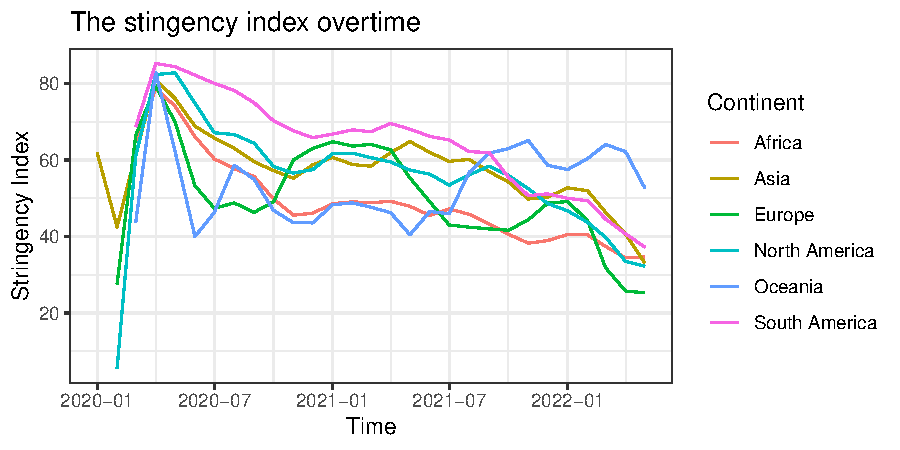
\includegraphics{report_files/figure-latex/stringency-index-1} 

}

\caption{The Stringency Index overtime for each Continent}\label{fig:stringency-index}
\end{figure}

From Figure \ref{fig:stringency-index} we can see that each continent has a response to COVID-19 at a different time. Asia continent is the first continent to have the restriction, this is because the COVID-19 was first identified in China which is in Asia. Then the WHO (\textcite{who}) declared COVID-19 as a public health emergency of international concern on 30 January 2020, that is when we can see that other continents start to apply the restriction. Then on 11 March 2020 WHO assessed that COVID-19 could be characterized as a pandemic that is the month before we see the spike in the stringency index. As mentioned in the section above, there is three outbreak in the plot, every time there is a COVID-19 outbreak the stringency index also increases.

\clearpage

\subsection*{Effect of restriction on the total number of COVID cases}

\begin{figure}

{\centering 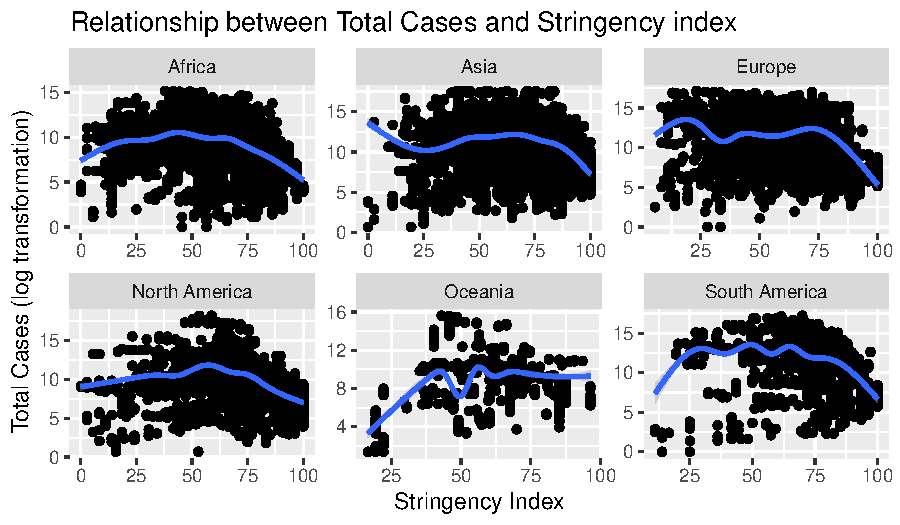
\includegraphics{report_files/figure-latex/relationship-tot-index-1} 

}

\caption{Relationship between total cases(log transformed) and stringency index}\label{fig:relationship-tot-index}
\end{figure}

We used log transformation on the number of cases to transform the skewed data. In Figure \ref{fig:relationship-tot-index}, we can see that there is a non-linear relationship between total cases and stringency index. The total case number keeps climbing even after implementing the restriction. Then it dropped as the restriction get stricter. This is because most of the time the government will start with the lower level of restriction but this won't have much effect on reducing the number of COVID-19 cases since the transmission of the COVID will occur before the lockdown started. Then, as the restriction increases and the longer people are staying at home, the number of total cases decreases. Therefore, we see the number of total cases climbing at first before the number goes down.

\clearpage

\hypertarget{how-do-positive-cases-change-relate-to-vaccination}{%
\subsection{\texorpdfstring{\textbf{How do positive cases change relate to vaccination?}}{How do positive cases change relate to vaccination?}}\label{how-do-positive-cases-change-relate-to-vaccination}}

\subsection*{Top 5 countries with highest daily new cases}

\begin{table}[!h]

\caption{\label{tab:table3}top 10 countries with highest daily cases}
\centering
\begin{tabular}[t]{lrr}
\toprule
location & mean\_daily\_cases & mean\_new\_vax\\
\midrule
\cellcolor{gray!6}{United States} & \cellcolor{gray!6}{120485} & \cellcolor{gray!6}{460807}\\
India & 70729 & 2008029\\
\cellcolor{gray!6}{France} & \cellcolor{gray!6}{56649} & \cellcolor{gray!6}{114808}\\
Germany & 50097 & 138851\\
\cellcolor{gray!6}{Brazil} & \cellcolor{gray!6}{46861} & \cellcolor{gray!6}{372420}\\
\addlinespace
South Korea & 39991 & 102167\\
\cellcolor{gray!6}{United Kingdom} & \cellcolor{gray!6}{38446} & \cellcolor{gray!6}{110154}\\
Italy & 30754 & 102214\\
\cellcolor{gray!6}{Russia} & \cellcolor{gray!6}{29095} & \cellcolor{gray!6}{203228}\\
Turkey & 27831 & 119240\\
\bottomrule
\end{tabular}
\end{table}

\subsection*{Trend of trend of new cases vs fully vaccinated}

\begin{figure}

{\centering 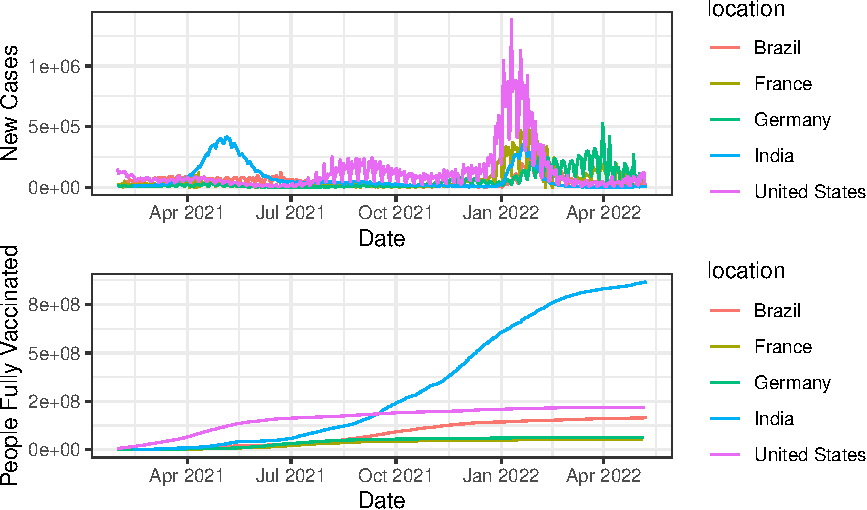
\includegraphics{report_files/figure-latex/figure4-1} 

}

\caption{trend of new cases vs fully vaccinated}\label{fig:figure4}
\end{figure}

\clearpage

\subsection*{Trend of trend of new cases vs fully vaccinated}

\begin{figure}

{\centering 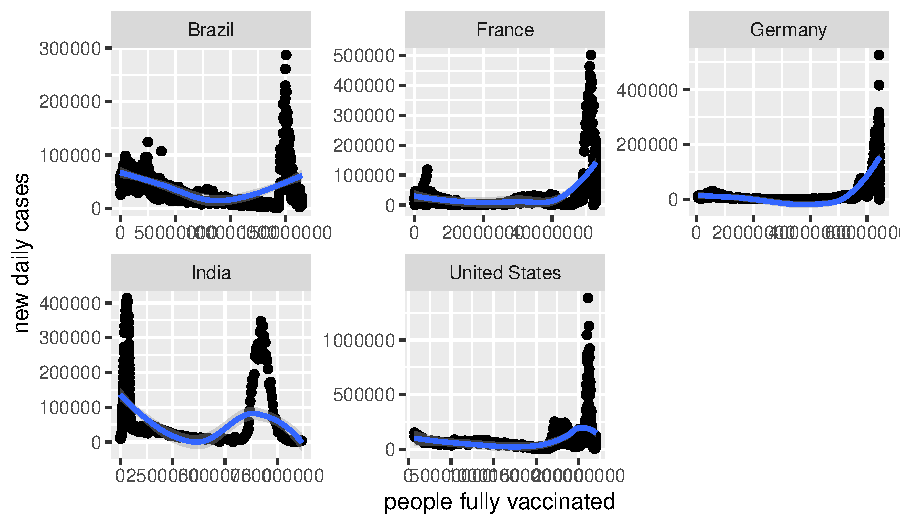
\includegraphics{report_files/figure-latex/figure5-1} 

}

\caption{correlation between new cases vs fully vaccinated}\label{fig:figure5}
\end{figure}

We sorted out countries by the order of mean new daily cases, referring \ref{tab:table3}, the table showcases top 10 countries with highest mean value of daily cases, our research onward will based on the top 5 countries, US, Brazil, India, Germany, France. From table \ref{tab:table3}, United States has the highest daily cases and India did the best in terms of vaccination.

Line chart \ref{fig:figure4} showcases the trend of new cases and fully vaccinated people from 2021 to latest data, and from the line chart, there is no corresponding effect between them. \textcite{lipsitch2020understanding} mentioned that the effectiveness of vaccination varies within different condition of health, however, both direct and indirect protection reduce virus symptoms generally.

Plot chart \ref{fig:figure5} was generate to explore relationship between vaccination and new cases, with vaccination on x axis, daily cases in y axis, the graph did not show significant correlation between them, smooth line was added to overview general movement. the graph further prove there is no expected higher vaccination with lower infections in the top 5 countries. \textcite{chen2021prediction} discussed the how mutation reduce the effectiveness of vaccination in terms of infection protection, and the research team mentioned we need to develop vaccine to deal with predicted mutation.

\clearpage

\hypertarget{how-do-death-rates-from-covid-19-differ-between-people-who-are-vaccinated-and-those-who-are-not}{%
\subsection{\texorpdfstring{\textbf{How do death rates from COVID-19 differ between people who are vaccinated and those who are not}}{How do death rates from COVID-19 differ between people who are vaccinated and those who are not}}\label{how-do-death-rates-from-covid-19-differ-between-people-who-are-vaccinated-and-those-who-are-not}}

\begin{table}[!h]

\caption{\label{tab:table}Average daily vaccinations and deaths for the countries with highest death rates.}
\centering
\begin{tabular}[t]{l|r|r}
\hline
location & average\_vaccinations\_per\_day & average\_deaths\_per\_day\\
\hline
\cellcolor{gray!6}{United States} & \cellcolor{gray!6}{1135290} & \cellcolor{gray!6}{1246}\\
\hline
Brazil & 934008 & 847\\
\hline
\cellcolor{gray!6}{India} & \cellcolor{gray!6}{4057187} & \cellcolor{gray!6}{657}\\
\hline
Russia & 434410 & 472\\
\hline
\cellcolor{gray!6}{Mexico} & \cellcolor{gray!6}{444551} & \cellcolor{gray!6}{407}\\
\hline
\end{tabular}
\end{table}

Table \ref{tab:table} shows the average daily vaccinations and deaths for the countries with highest death rates. We can see that \textbf{United States} has the highest deaths per day of \emph{1264} while \textbf{India} has the highest average vaccinations per day of approx \emph{4057187}.

\begin{figure}

{\centering 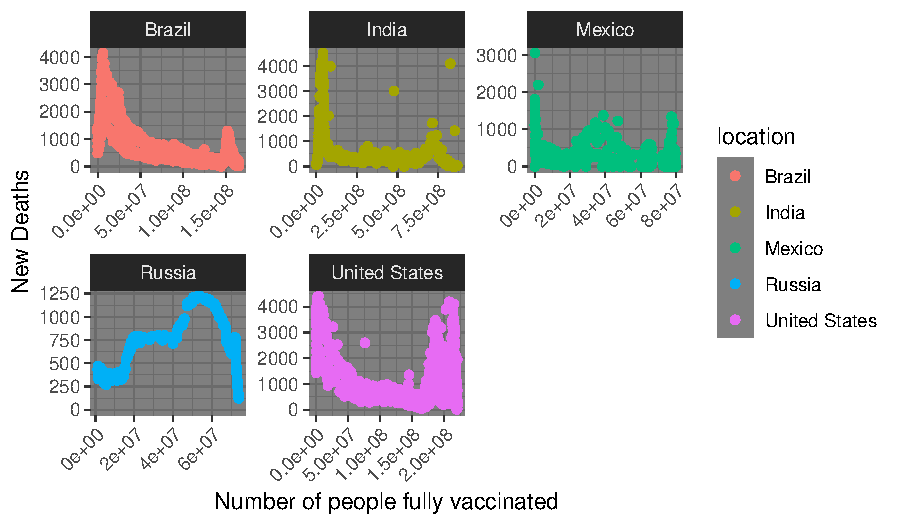
\includegraphics{report_files/figure-latex/graph-1} 

}

\caption{Relationship between new deaths and vaccination status }\label{fig:graph}
\end{figure}

From the figure \ref{fig:graph} we can clearly see that in countries like Brazil, India and Mexico, there is a clear effect of vaccinations on the death rates. The death rates in the third wave (second peak of the graph) have fallen to around 25\% of what they were in the second wave (first peak of the graph).

\clearpage

For the countries like Russia and United States the case is a little different as the vaccinations have increased but the number of deaths due to COVID-19 have remained constant or have increased. This may be due to many reasons such as the vaccine that was being used in the particular country, the immunity of the individual at the given location and the other Comorbidities they had. Also, the vaccine was designed using the first strain of COVID-19 virus and mutations caused in the virus might have affected the efficacy of the vaccine.

A research published \textcite{paper} also confirmed that double vaccination against COVID-19 will decrease the death rate by 74.89 \%

\hypertarget{conclusion}{%
\section{\texorpdfstring{\textbf{CONCLUSION}}{CONCLUSION}}\label{conclusion}}

Globally, after the decline in the number of total cases since the end of March 2022, new daily COVID-19 cases have stabilized in the latest weeks and the number of deaths continues to decline. The introduction of Vaccines in 2021, raises the question of whether restrictions will still be effective against the spread of the COVID-19. In this report we can see that the restriction policies can reduce the spread of the virus, however, this method does not have an immediate effect as the spread occurs before the restriction. We also found that the vaccination seems to not affect the spread of the virus due to the mutation. It is clear that vaccination against COVID-19 is not the best method to reduce the number of cases but it is still one of the best and safest ways to reduces the number of deaths.

\clearpage

\printbibliography

\end{document}

